% Options for packages loaded elsewhere
\PassOptionsToPackage{unicode}{hyperref}
\PassOptionsToPackage{hyphens}{url}
%
\documentclass[
  11pt,
  twoside,
  11pt]{article}
\usepackage{amsmath,amssymb}
\usepackage{iftex}
\ifPDFTeX
  \usepackage[T1]{fontenc}
  \usepackage[utf8]{inputenc}
  \usepackage{textcomp} % provide euro and other symbols
\else % if luatex or xetex
  \usepackage{unicode-math} % this also loads fontspec
  \defaultfontfeatures{Scale=MatchLowercase}
  \defaultfontfeatures[\rmfamily]{Ligatures=TeX,Scale=1}
\fi
\usepackage{lmodern}
\ifPDFTeX\else
  % xetex/luatex font selection
\fi
% Use upquote if available, for straight quotes in verbatim environments
\IfFileExists{upquote.sty}{\usepackage{upquote}}{}
\IfFileExists{microtype.sty}{% use microtype if available
  \usepackage[]{microtype}
  \UseMicrotypeSet[protrusion]{basicmath} % disable protrusion for tt fonts
}{}
\makeatletter
\@ifundefined{KOMAClassName}{% if non-KOMA class
  \IfFileExists{parskip.sty}{%
    \usepackage{parskip}
  }{% else
    \setlength{\parindent}{0pt}
    \setlength{\parskip}{6pt plus 2pt minus 1pt}}
}{% if KOMA class
  \KOMAoptions{parskip=half}}
\makeatother
\usepackage{xcolor}
\usepackage{color}
\usepackage{fancyvrb}
\newcommand{\VerbBar}{|}
\newcommand{\VERB}{\Verb[commandchars=\\\{\}]}
\DefineVerbatimEnvironment{Highlighting}{Verbatim}{commandchars=\\\{\}}
% Add ',fontsize=\small' for more characters per line
\usepackage{framed}
\definecolor{shadecolor}{RGB}{248,248,248}
\newenvironment{Shaded}{\begin{snugshade}}{\end{snugshade}}
\newcommand{\AlertTok}[1]{\textcolor[rgb]{0.94,0.16,0.16}{#1}}
\newcommand{\AnnotationTok}[1]{\textcolor[rgb]{0.56,0.35,0.01}{\textbf{\textit{#1}}}}
\newcommand{\AttributeTok}[1]{\textcolor[rgb]{0.13,0.29,0.53}{#1}}
\newcommand{\BaseNTok}[1]{\textcolor[rgb]{0.00,0.00,0.81}{#1}}
\newcommand{\BuiltInTok}[1]{#1}
\newcommand{\CharTok}[1]{\textcolor[rgb]{0.31,0.60,0.02}{#1}}
\newcommand{\CommentTok}[1]{\textcolor[rgb]{0.56,0.35,0.01}{\textit{#1}}}
\newcommand{\CommentVarTok}[1]{\textcolor[rgb]{0.56,0.35,0.01}{\textbf{\textit{#1}}}}
\newcommand{\ConstantTok}[1]{\textcolor[rgb]{0.56,0.35,0.01}{#1}}
\newcommand{\ControlFlowTok}[1]{\textcolor[rgb]{0.13,0.29,0.53}{\textbf{#1}}}
\newcommand{\DataTypeTok}[1]{\textcolor[rgb]{0.13,0.29,0.53}{#1}}
\newcommand{\DecValTok}[1]{\textcolor[rgb]{0.00,0.00,0.81}{#1}}
\newcommand{\DocumentationTok}[1]{\textcolor[rgb]{0.56,0.35,0.01}{\textbf{\textit{#1}}}}
\newcommand{\ErrorTok}[1]{\textcolor[rgb]{0.64,0.00,0.00}{\textbf{#1}}}
\newcommand{\ExtensionTok}[1]{#1}
\newcommand{\FloatTok}[1]{\textcolor[rgb]{0.00,0.00,0.81}{#1}}
\newcommand{\FunctionTok}[1]{\textcolor[rgb]{0.13,0.29,0.53}{\textbf{#1}}}
\newcommand{\ImportTok}[1]{#1}
\newcommand{\InformationTok}[1]{\textcolor[rgb]{0.56,0.35,0.01}{\textbf{\textit{#1}}}}
\newcommand{\KeywordTok}[1]{\textcolor[rgb]{0.13,0.29,0.53}{\textbf{#1}}}
\newcommand{\NormalTok}[1]{#1}
\newcommand{\OperatorTok}[1]{\textcolor[rgb]{0.81,0.36,0.00}{\textbf{#1}}}
\newcommand{\OtherTok}[1]{\textcolor[rgb]{0.56,0.35,0.01}{#1}}
\newcommand{\PreprocessorTok}[1]{\textcolor[rgb]{0.56,0.35,0.01}{\textit{#1}}}
\newcommand{\RegionMarkerTok}[1]{#1}
\newcommand{\SpecialCharTok}[1]{\textcolor[rgb]{0.81,0.36,0.00}{\textbf{#1}}}
\newcommand{\SpecialStringTok}[1]{\textcolor[rgb]{0.31,0.60,0.02}{#1}}
\newcommand{\StringTok}[1]{\textcolor[rgb]{0.31,0.60,0.02}{#1}}
\newcommand{\VariableTok}[1]{\textcolor[rgb]{0.00,0.00,0.00}{#1}}
\newcommand{\VerbatimStringTok}[1]{\textcolor[rgb]{0.31,0.60,0.02}{#1}}
\newcommand{\WarningTok}[1]{\textcolor[rgb]{0.56,0.35,0.01}{\textbf{\textit{#1}}}}
\usepackage{longtable,booktabs,array}
\usepackage{calc} % for calculating minipage widths
% Correct order of tables after \paragraph or \subparagraph
\usepackage{etoolbox}
\makeatletter
\patchcmd\longtable{\par}{\if@noskipsec\mbox{}\fi\par}{}{}
\makeatother
% Allow footnotes in longtable head/foot
\IfFileExists{footnotehyper.sty}{\usepackage{footnotehyper}}{\usepackage{footnote}}
\makesavenoteenv{longtable}
\usepackage{graphicx}
\makeatletter
\def\maxwidth{\ifdim\Gin@nat@width>\linewidth\linewidth\else\Gin@nat@width\fi}
\def\maxheight{\ifdim\Gin@nat@height>\textheight\textheight\else\Gin@nat@height\fi}
\makeatother
% Scale images if necessary, so that they will not overflow the page
% margins by default, and it is still possible to overwrite the defaults
% using explicit options in \includegraphics[width, height, ...]{}
\setkeys{Gin}{width=\maxwidth,height=\maxheight,keepaspectratio}
% Set default figure placement to htbp
\makeatletter
\def\fps@figure{htbp}
\makeatother
\setlength{\emergencystretch}{3em} % prevent overfull lines
\providecommand{\tightlist}{%
  \setlength{\itemsep}{0pt}\setlength{\parskip}{0pt}}
\setcounter{secnumdepth}{5}
\usepackage{geometry}
\usepackage{enumerate}
\usepackage{latexsym,booktabs}
\usepackage{amsmath,amssymb}
\usepackage{graphicx}
\usepackage{hyperref}
\usepackage[singlespacing]{setspace}
\usepackage{calc}
\geometry{a4paper,left=2cm,right=2.0cm, top=2cm, bottom=2.0cm}
\usepackage{booktabs}
\usepackage{longtable}
\usepackage{array}
\usepackage{multirow}
\usepackage{wrapfig}
\usepackage{float}
\usepackage{colortbl}
\usepackage{pdflscape}
\usepackage{tabu}
\usepackage{threeparttable}
\usepackage{threeparttablex}
\usepackage[normalem]{ulem}
\usepackage{makecell}
\usepackage{xcolor}
\newtheorem{Definition}{Definition}
\newtheorem{Theorem}{Theorem}
\newtheorem{Lemma}{Lemma}
\newtheorem{Corollary}{Corollary}
\newtheorem{Proposition}{Proposition}
\newtheorem{Algorithm}{Algorithm}
\numberwithin{Theorem}{section}
\numberwithin{Definition}{section}
\numberwithin{Lemma}{section}
\numberwithin{Algorithm}{section}
\numberwithin{equation}{section}
\newcommand{\dottedline}[1]{\makebox[#1]{.\dotfill}}
\usepackage{booktabs}
\usepackage{longtable}
\usepackage{array}
\usepackage{multirow}
\usepackage{wrapfig}
\usepackage{float}
\usepackage{colortbl}
\usepackage{pdflscape}
\usepackage{tabu}
\usepackage{threeparttable}
\usepackage{threeparttablex}
\usepackage[normalem]{ulem}
\usepackage{makecell}
\usepackage{xcolor}
\ifLuaTeX
  \usepackage{selnolig}  % disable illegal ligatures
\fi
\IfFileExists{bookmark.sty}{\usepackage{bookmark}}{\usepackage{hyperref}}
\IfFileExists{xurl.sty}{\usepackage{xurl}}{} % add URL line breaks if available
\urlstyle{same}
\hypersetup{
  hidelinks,
  pdfcreator={LaTeX via pandoc}}

\author{}
\date{\vspace{-2.5em}}

\begin{document}

\pagestyle{empty}

% =============================================================================
% Title page
% =============================================================================
\begin{titlepage}
\vspace*{.5em}
\center
\textbf{\Large{The School of Mathematics}} \\
\vspace*{1em}
\begin{figure}[!h]
\centering

\includegraphics[width=180pt]{CentredLogoCMYK.jpg}
\end{figure}
\vspace{2em}
\textbf{\Huge{My Incredible Thesis}}\\[2em]
\textbf{\LARGE{by}}\\
\vspace{2em}
\textbf{\LARGE{My Name}}\\
\vspace{6.5em}
\Large{Dissertation Presented for the Degree of\\
MSc in Statistics with Data Science}\\
\vspace{6.5em}
\Large{July 2021}\\
\vspace{3em}
\Large{Supervised by\\Dr Very Important and Dr Strangelove}
\vfill
\end{titlepage}

\cleardoublepage

% =============================================================================
% Executive summary, acknowledgments, and own work declaration
% =============================================================================
\begin{center}
\Large{Executive Summary}
\end{center}

Here comes your executive summary ...

\clearpage

\begin{center}
\Large{Acknowledgments}
\end{center}

Here come your acknowledgments ...

\clearpage

\begin{center}
\Large{University of Edinburgh – Own Work Declaration}
\end{center}


This sheet must be filled in, signed and dated - your work will not be marked unless this is done.
% Replace the commands \dottedline{8cm}, %\dottedline{6cm}, etc. with you name, Matriculation 
% Number, etc.
\vspace{1cm}

Name: \dottedline{8cm}

Matriculation Number: \dottedline{6cm}

Title of work: \dottedline{8cm}

\vspace{1cm}

I confirm that all this work is my own except where indicated, and that I have:
\begin{itemize}
\item   Clearly referenced/listed all sources as appropriate                    
\item   Referenced and put in inverted commas all quoted text (from books, web, etc)    
\item   Given the sources of all pictures, data etc. that are not my own                
\item   Not made any use of the report(s) or essay(s) of any other student(s) either past   
or present  
\item   Not sought or used the help of any external professional academic agencies for the work
\item   Acknowledged in appropriate places any help that I have received from others    (e.g. fellow students, technicians, statisticians, external sources)
\item   Complied with any other plagiarism criteria specified in the Course handbook
\end{itemize}

I understand that any false claim for this work will be penalised in accordance with
the University regulations  (\url{https://teaching.maths.ed.ac.uk/main/msc-students/msc-programmes/statistics/data-science/assessment/academic-misconduct}).                                

\vspace{1cm}

Signature \dottedline{8cm}

%Include your signature as an image with the
%\includegraphics command 
%(see an example later in the document)

\vspace{5mm}

Date \dottedline{8cm}


\clearpage



% =============================================================================
% Table of contents, tables, and pictures (if applicable)
% =============================================================================
\pagestyle{plain}
\setcounter{page}{1}
\pagenumbering{Roman}
\tableofcontents
\clearpage
\listoftables
\listoffigures
\cleardoublepage

\pagenumbering{arabic}
\setcounter{page}{1}

\nocite{*}
\bibliographystyle{abbrv}
\clearpage

\section{Introduction}
\label{sec:intro}

Here I will write a very good, precise and brief introduction.
Particularly Section \ref{sec:methods} is good!
\clearpage

\section{Methods}
\label{sec:methods}
In the following, I explain what did I do and how.

I should really cut this short, but BlaBlaBlaBla BlaBlaBlaBlaBla Bla Bla BlaBlaBla Bla Bla BlaBlaBla Bla BlaBla BlaBla Bla BlaBlaBlaBla Bla BlaBla Bla Bla Bla BlaBla BlaBlaBlaBla BlaBlaBlaBlaBla Bla Bla BlaBlaBla Bla. Bla BlaBlaBla Bla BlaBla BlaBla Bla BlaBlaBlaBla Bla BlaBla Bla Bla Bla BlaBla BlaBlaBlaBla. BlaBlaBlaBlaBla Bla Bla BlaBlaBla Bla Bla BlaBlaBla Bla BlaBla BlaBla Bla BlaBlaBlaBla Bla BlaBla Bla Bla Bla BlaBla BlaBlaBlaBla BlaBlaBlaBlaBla Bla Bla BlaBlaBla Bla Bla BlaBlaBla Bla BlaBla BlaBla Bla BlaBlaBlaBla Bla BlaBla Bla Bla Bla BlaBla BlaBlaBlaBla BlaBlaBlaBlaBla Bla Bla BlaBlaBla Bla Bla BlaBlaBla Bla BlaBla BlaBla Bla. BlaBlaBlaBla Bla BlaBla Bla Bla Bla BlaBla BlaBlaBlaBla BlaBlaBlaBlaBla Bla Bla BlaBlaBla Bla Bla BlaBlaBla Bla BlaBla BlaBla Bla BlaBlaBlaBla Bla BlaBla Bla Bla Bla BlaBla.
% You can enter comments in LaTeX
% like this.

When you write outside of the LaTeX environment, you can use Markdown syntax. Some R Markdown basics: \url{https://rmarkdown.rstudio.com/authoring_basics.html}.

More in depth explanation is available in the book \emph{RMarkdown for Scientists}:\\
\url{https://rmd4sci.njtierney.com}.

Note that I start a new paragraph when I have an empty line like this. BlaBlaBlaBla BlaBlaBlaBlaBla Bla Bla BlaBlaBla Bla Bla BlaBlaBla Bla BlaBla BlaBla Bla BlaBlaBlaBla Bla BlaBla Bla Bla Bla. BlaBla BlaBlaBlaBla BlaBlaBlaBlaBla Bla Bla BlaBlaBla Bla Bla BlaBlaBla Bla BlaBla BlaBla Bla BlaBlaBlaBla Bla BlaBla Bla Bla Bla BlaBla BlaBlaBlaBla BlaBlaBlaBlaBla Bla Bla BlaBlaBla Bla Bla BlaBlaBla. Bla BlaBla BlaBla Bla BlaBlaBlaBla Bla BlaBla Bla Bla Bla BlaBla BlaBlaBlaBla BlaBlaBlaBlaBla Bla Bla BlaBlaBla Bla Bla BlaBlaBla Bla. BlaBla BlaBla Bla BlaBlaBlaBla Bla BlaBla Bla Bla Bla BlaBla BlaBlaBlaBla BlaBlaBlaBlaBla Bla Bla BlaBlaBla Bla Bla BlaBlaBla Bla BlaBla BlaBla Bla BlaBlaBlaBla Bla BlaBla Bla Bla Bla BlaBla.

But I can also end a line with an empty line. You can enter display formulas like this using Latex syntax in the formula: \[
E = mc^2
\] You can also enter in-line formulas like \(c^2=a^2+b^2\) using LaTeX syntax.

\newpage

\subsection{Models}
\label{sec:Models}

Models are \emph{very} helpful because.
\begin{itemize}
 \item They're good.
 \item They're helpful.
\end{itemize}
\clearpage

\subsection{Techniques}
\label{sec:Techniques}

Techniques even better because.
\begin{enumerate}
 \item They're magnificent.
 \item If they work.
\end{enumerate}
\clearpage

\section{Results}
\label{sec:results}
I this section, I explain what did I discover.

Now it's getting very technical \ldots{} I will cite \cite{shiina,groewe2001}. I will also show my incredible $\alpha$, $\beta$ and $\gamma$ mathematics and do some other fancy stuff.

\subsection{Formulae}

For example look at this
\begin{equation}\label{eqn:aProblem}
\min{}\sum_{s\in\mathcal{S}}Pr_{s}\left[\sum_{t=1}^{T}\left(
\sum_{g\in\mathcal{G}}\left(\alpha_{gts}C_{g}^{0}+
p_{gts}C_{g}^{1}+\left(p_{gts}\right)^{2}C_{g}^{2}\right)
+\sum_{g\in\mathcal{C}}\gamma_{gts}C_{g}^{s}\right)\right],
\end{equation}
and you will see that it has a little number on the side so that I can refer to it as equation (\ref{eqn:aProblem}). Now if I do this
\begin{eqnarray}
\sum_{i=1}^{n}k_{i}&=&20\label{eqn:one}\\
\sum_{j=20}^{m}\delta_{i}&\geq{}&\eta{}\notag
\end{eqnarray}
I can align two formulae and control which one has a number on the side. It is (\ref{eqn:one}). I can also do something like this
\begin{displaymath}
Y_{l}=\left[\begin{array}{cc}
             \left(y_{s}+i\frac{b_{c}}{2}\right)\frac{1}{\tau{}^{2}} &
             -y_{s}\frac{1}{\tau{}e^{-i\theta^{s}}}\\
             -y_{s}\frac{1}{\tau{}e^{i\theta^{s}}} &
             y_{s}+i\frac{b_{c}}{2}
             \end{array}\right],
\end{displaymath}
and it won't have a number on the side. Now if I have to do some huge mathematics I'd better structure it a little and include linebreaks etc. so that it fits on one page.
\begin{eqnarray}\label{eqn:horrible}
p_{l}^{f}&=&G_{l11}\left(2v_{F(l)}\bar{v}_{F(l)}-\bar{v}_{F(l)}^{2}\right)\\
&+&
\bar{v}_{F(l)}\bar{v}_{T(l)}
\left[
B_{l12}\sin{}(\bar{\delta{}}_{F(l)}-\bar{\delta{}}_{T(l)})
+G_{l12}\cos{}(\bar{\delta{}}_{F(l)}-\bar{\delta{}}_{T(l)})
\right]\notag\\
&+&
\left[\begin{array}{r}
      \bar{v}_{T(l)}
      \left[
      B_{l12}\sin{}(\bar{\delta{}}_{F(l)}-\bar{\delta{}}_{T(l)})
      +G_{l12}\cos{}(\bar{\delta{}}_{F(l)}-\bar{\delta{}}_{T(l)})
      \right]\\
      \bar{v}_{F(l)}
      \left[
      B_{l12}\sin{}(\bar{\delta{}}_{F(l)}-\bar{\delta{}}_{T(l)})
      +G_{l12}\cos{}(\bar{\delta{}}_{F(l)}-\bar{\delta{}}_{T(l)})
      \right]\\
      \bar{v}_{F(l)}\bar{v}_{T(l)}
      \left[
      B_{l12}\cos{}(\bar{\delta{}}_{F(l)}-\bar{\delta{}}_{T(l)})
      -G_{l12}\sin{}(\bar{\delta{}}_{F(l)}-\bar{\delta{}}_{T(l)})
      \right]\\
      \bar{v}_{F(l)}\bar{v}_{T(l)}
      \left[
      -B_{l12}\cos{}(\bar{\delta{}}_{F(l)}-\bar{\delta{}}_{T(l)})
      +G_{l12}\sin{}(\bar{\delta{}}_{F(l)}-\bar{\delta{}}_{T(l)})
      \right]\\
      \end{array}\right]
\cdot{}
\left[\begin{array}{c}
      v_{F(l)}-\bar{v}_{F(l)}\\
      v_{T(l)}-\bar{v}_{T(l)}\\
      \delta_{F(l)}-\bar{\delta{}}_{F(l)}\\
      \delta_{T(l)}-\bar{\delta{}}_{T(l)}
      \end{array}\right],\notag
\end{eqnarray}
This is a lot of fun!
\clearpage

\subsection{Important Things}
Finally we should have a nice picture like this one. However, I won't forget that figures and table are environments which float around in my document. So LaTeX will place them wherever it thinks they fit well with the surrounding text. I can try to change that with a float specifier, e.g. [!ht].
%This is a comment. The Compiler ignores it. It is here to remind me that, if I use a .jpeg or .png picture file as below I will need to compile the document with the pdflatex compiler.
\begin{figure}[!ht]
\centering
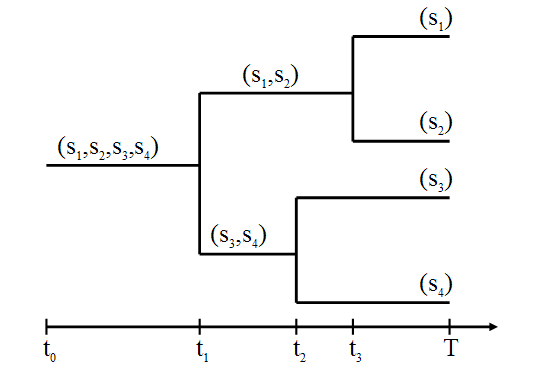
\includegraphics[width=0.5\textwidth]{scenTree.png}
\caption{Look at this scenario tree with funny times $t_{1}$ and scenarios $s_{1}$ etc.}
\label{fig:scenarioTree}
\end{figure}
Now I want to use one of my own environments. I want to define something.
\begin{Definition}
 I define
$$
\Gamma_{\eta}:=\sum_{i=1}^{n}\sum_{j=i}^{n}\xi{}(i,j)
$$
\end{Definition}
I definitely need some good tables, so I do this.
\begin{table}[!ht]
\centering
\begin{tabular}{|ll|rrrr|}
\hline
Case&Generators&Therm. Units&Lines&Peak load: [MW]&[MVar]\\
\hline\hline
6 bus&3 at 3 buses&2&11&210&210\\
9 bus&3 at 3 buses&3&9&315&115\\
24 bus&33 at 11 buses&26&38&2850&580\\
30 bus&6 at 6 buses&5&41&189.2&107.2\\
39 bus&10 at 10 buses&7&46&6254.2&1387.1\\
57 bus&7 at 7 buses&7&80&1250.8&336.4\\
\hline
\end{tabular}
\caption{Something that doesn't make sense.}
\label{tab:things}
\end{table}
I should really refer to Table \ref{tab:things}.

\subsection{And now something else}

\noindent
Let:
\begin{eqnarray*}
\Omega_0 & = & \{(x,y,z,f): \text{ satisfying } (9)-(19)\}, \\
\Omega_1 & = & \{(x,y,z,f): \text{ satisfying } (9),(11)-(20)\}, \\
\overline{\Omega}_0 & = & \{\textbf{0}\leq (x,y,z,f) \leq \textbf{1}: \text{ satisfying } (9)-(18)\}, \\
\overline{\Omega}_1 & = & \{\textbf{0}\leq (x,y,z,f) \leq \textbf{1}: \text{ satisfying } (9),(11)-(18),(20)\} \,.
\end{eqnarray*}
%
where $\textbf{0}$ and $\textbf{1}$ are vectors of appropriate dimensions with 0's and 1's, respectively.
Next we see that both $\Omega_0$ and $\Omega_1$ give equivalent formulations for the A-MSSP. In particular, the following statements hold:

\begin{Proposition}
$\Omega_0 \subseteq \Omega_1$.
\end{Proposition}

\noindent
\textbf{Proof.}
Let us suppose there exists $(x,y,z,f) \in \Omega_1$ such that $(x,y,z,f) \notin \Omega_0$.
Then, there exist indices $i \in I$ and $t \in \{0,\ldots,|T|-s_i\} $ with $x_i^t > \displaystyle 0.5\,\left( \sum_{h=1}^{s_i} x_i^{t+h} +1\right)$.
By definition, $x_i^t = 1$ and $x_i^{t+h} = 0$ for all $h \in \{1,\dots,s_i\}$. By~(11) and (12), $\displaystyle \sum_{h=1}^{s_i} f_i^{th}=1$, so $f_i^{th'}=1$ for some $h' \in \{1,\dots,s_i\}$.
But then,
\[ 0 \:=\: x_i^{t+h'} \:=\: \sum_{h=\max \{1, t+h'-(|T|-s_i)\}}^{\min\{s_i,t+h'\}} f_i^{t+h'-h,h} \:\ge\: f_i^{th'} \:=\: 1 \,,
\]
as $h' \in [\max \{1, t+h'-(|T|-s_i)\}, \min\{s_i,t+h'\}]$.
\hfill $\square$
\bigskip

\noindent
This immediately gives us
\begin{Corollary}
AS is a valid formulation for the A-MSSP.
\end{Corollary}

\noindent
Next we compare the Linear Programming (LP) relaxations of the two formulations.

\begin{Proposition}
$\overline{\Omega}_1 \subseteq  \overline{\Omega}_0 $.
\end{Proposition}

\noindent
\textbf{Proof.}
Homework
\hfill $\square$
\clearpage

\hypertarget{sec:IncludingMarkdown}{%
\subsection{Including Markdown and R code}\label{sec:IncludingMarkdown}}

This subsection is called Section \ref{sec:IncludingMarkdown}.

Even from LaTeX, this subsection is still called Section \ref{sec:IncludingMarkdown}.

Markdown is a simple formatting syntax for authoring HTML, PDF, and MS Word documents. For more details on using R Markdown see \url{http://rmarkdown.rstudio.com}.

When you click the \textbf{Knit} button a document will be generated that includes both content as well as the output of any embedded R code chunks within the document. You can embed an R code chunk like this:

\begin{Shaded}
\begin{Highlighting}[]
\FunctionTok{summary}\NormalTok{(cars)}
\end{Highlighting}
\end{Shaded}

\begin{verbatim}
##      speed           dist       
##  Min.   : 4.0   Min.   :  2.00  
##  1st Qu.:12.0   1st Qu.: 26.00  
##  Median :15.0   Median : 36.00  
##  Mean   :15.4   Mean   : 42.98  
##  3rd Qu.:19.0   3rd Qu.: 56.00  
##  Max.   :25.0   Max.   :120.00
\end{verbatim}

You can also embed plots, for example:

\begin{figure}
\centering
\includegraphics{SwDS_template_files/figure-latex/pressure-plot-1.pdf}
\caption{\label{fig:pressure-plot}An amazing plot}
\end{figure}

In the above R code chunk, \texttt{pressure-plot} is the chunk name. Note that the \texttt{echo\ =\ print.all.code} parameter was added to the code chunk to potentially prevent printing of the R code that generated the plot (by default, \texttt{print.all.code=FALSE}, but this can be changed at the beginning of the document to display all of the code).

We can reference the pressure plot within a Markdown chunk as Figure \ref{fig:pressure-plot}.

We can reference the pressure plot within a LaTeX chunk as Figure \ref{fig:pressure-plot}.

\begin{table}

\caption{\label{tab:MtcarsTable1}Table in plain LaTeX format}
\centering
\begin{tabular}[t]{l|r|r|r|r|r|r}
\hline
  & mpg & cyl & disp & hp & drat & wt\\
\hline
Mazda RX4 & 21.0 & 6 & 160 & 110 & 3.90 & 2.620\\
\hline
Mazda RX4 Wag & 21.0 & 6 & 160 & 110 & 3.90 & 2.875\\
\hline
Datsun 710 & 22.8 & 4 & 108 & 93 & 3.85 & 2.320\\
\hline
Hornet 4 Drive & 21.4 & 6 & 258 & 110 & 3.08 & 3.215\\
\hline
Hornet Sportabout & 18.7 & 8 & 360 & 175 & 3.15 & 3.440\\
\hline
\end{tabular}
\end{table}

\begin{table}

\caption{\label{tab:MtcarsTable2}Table with booktabs}
\centering
\begin{tabular}[t]{lrrrrrr}
\toprule
  & mpg & cyl & disp & hp & drat & wt\\
\midrule
Mazda RX4 & 21.0 & 6 & 160 & 110 & 3.90 & 2.620\\
Mazda RX4 Wag & 21.0 & 6 & 160 & 110 & 3.90 & 2.875\\
Datsun 710 & 22.8 & 4 & 108 & 93 & 3.85 & 2.320\\
Hornet 4 Drive & 21.4 & 6 & 258 & 110 & 3.08 & 3.215\\
Hornet Sportabout & 18.7 & 8 & 360 & 175 & 3.15 & 3.440\\
\bottomrule
\end{tabular}
\end{table}

We have two tables, Table \ref{tab:MtcarsTable1} and Table \ref{tab:MtcarsTable2}. Please make sure not to include dots (.) or other special characters in the names of the R code chunks (such as MtcarsTable2), as this may cause issues with the labels.

We can reference the two tables within a LaTeX chunk as Table \ref{tab:MtcarsTable1} and Table \ref{tab:MtcarsTable2}.

You can see more information on how to create nice tables in R Markdown at \url{https://haozhu233.github.io/kableExtra/awesome_table_in_pdf.pdf} and \url{https://rfortherestofus.com/2019/11/how-to-make-beautiful-tables-in-r/}.

\clearpage

\section{Conclusion}
\label{sec:conclusion}
In this section, I explain what what do my results mean.

I have no idea how to conclude, so I don't write much. But what follows is important.
\clearpage

%the entries have to be in the file literature.bib
\bibliography{literature}
\clearpage

\appendix
\section*{Appendices}
\addcontentsline{toc}{section}{Appendices}

\section{An Appendix}
\label{app:one}

Something.
\clearpage

\section{Another Appendix}
\label{app:two}

Something else.

\end{document}
